\documentclass[tikz]{standalone}
\usepackage[utf8]{inputenc}
\usepackage{tikz}

\begin{document}
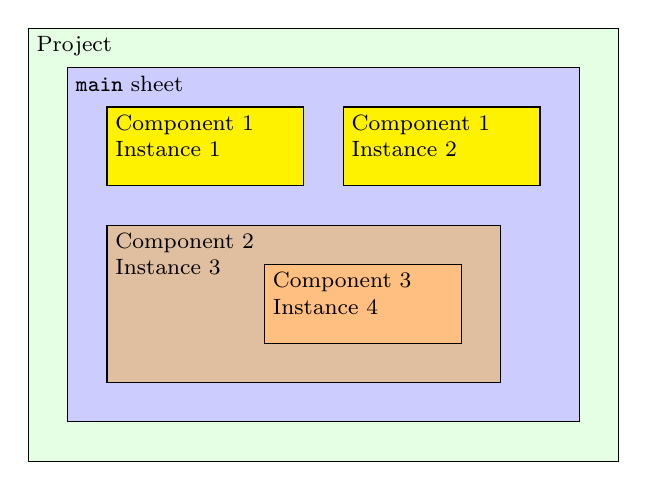
\begin{tikzpicture}
	\footnotesize
	\draw[fill=green!10]
	(0,0) node[below right]{Project}
	rectangle ++(7.5,-5.5);
	\draw[fill=blue!20]
	(0.5,-0.5) node[below right]{\texttt{main} sheet}
	rectangle ++(6.5,-4.5);
	\draw[fill=yellow]
	(1,-1) node[below right,align=left]{Component 1\\Instance 1}
	rectangle ++(2.5,-1)
	(4,-1) node[below right,align=left]{Component 1\\Instance 2}
	rectangle ++(2.5,-1);
	\draw[fill=brown!50]
	(1,-2.5) node[below right,align=left]{Component 2\\Instance 3}
	rectangle ++(5,-2);
	\draw[fill=orange!50]
	(3,-3) node[below right,align=left]{Component 3\\Instance 4}
	rectangle ++(2.5,-1)
	;

\end{tikzpicture}
\end{document}
